\chapter{Localization}\label{chap:localization}
Robots employ sensors and actuators that are subject to uncertainty. Chapter~\ref{chap:uncertainty} describes how to quantify this uncertainty using probability density functions that associate a probability with each possible outcome of a random process, such as the reading of a sensor or the actual physical change of an actuator. Here, the robot's pose is a compound metric that is of central importance to mobile robotics, and the focus of this chapter.


%One of the most common probability density functions is the Gaussian distribution. It has the shape of a bell and can entirely be described by its mean --- the center of the bell curve --- and its variance, the width of the bell curve.
There are many ways to localize a robot in its environment, and odometry is just one of them. A different possible way to localize a robot in its environment is to extract high-level features (Chapter~\ref{chap:feature_extraction}), such as the distance to a wall from a number of different sensors. %As the underlying measurements are uncertain, these measurements will be subject to uncertainty. How to calculate the uncertainty of a feature from the uncertainty of the sensors that detect this feature, is covered by the error propagation law. The key insight is that the variance of a feature is the weighted sum of all contributing sensors' variances, weighed by their impact on the feature of interest. This impact can be approximated by the derivative of the function that maps a sensor's input to the measurement of the feature.

As we have seen in \cref{chap:uncertainty}, uncertainty keeps propagating without the ability to take corrective measurements. The goals of this chapter are to present mathematical tools and algorithms that will enable you to actually shrink the uncertainty of a measurement by combining it with additional observations.  In particular, this chapter will cover
\begin{itemize}
    \item using landmarks to improve the accuracy of a discrete position estimate (Markov Localization and Bayes Filter),
    \item approximating continuous position estimates (Particle Filter),
    \item using the Extended Kalman Filter to estimate a continuous position estimate.
\end{itemize}

\section{Motivating Example}
Imagine a floor with three doors, two of which are closer together, and the third farther down the corridor (\cref{fig:three_door_example}). Imagine now that your robot is able to detect doors, namely that it is able to tell whether it is in front of a wall or in front of a door. Features like this can serve as a landmark for the robot. Given a map of this simple environment and no information whatsoever about where our robot is located, we can use landmarks to drastically reduce the space of possible locations once the robot has passed one of the doors. One way of representing this belief is to describe the robot's position with three Gaussian distributions, each centered in front of a door and its variance a function of the uncertainty with which the robot can detect a door's center. This is known as a multi-hypothesis belief, since we have a hypothesis stating that the robot can be in front of each door. What happens if the robot continues to move? From the error propagation law we know:
\begin{enumerate}
\item The Gaussians describing the robot's 3 possible locations will move with the robot.
\item The variance of each Gaussian will keep increasing with the distance the robot moves.
\end{enumerate}
What happens if the robot arrives at another door? Given a map of the environment, we can now map the three Gaussian distributions to the location of the three doors. As all three Gaussians will have moved, but the doors are not equally spaced, only some of the peaks will coincide with the location of  a door. Assuming we trust our door detector much more than our odometry estimate, we can now remove all beliefs that do not coincide with a door. Again assuming our door detector can detect the center of a door with some accuracy, our location estimate's uncertainty is now only limited by that of the door detector.


Things are just slightly more complicated if our door detector is also subject to uncertainty: there is a chance that we are in front of a door, but haven't noticed it. Then, it would be a mistake to remove this belief. Instead, we just weigh all beliefs with the probability that there \textsl{could} be a door. Say our door detector detects false-positives with a 10\% chance. Then, there is a 10\% chance to be at any location that is not in front of a door, even if our detector tells us we are in front of a door. Similarly, our detector might detect false-negatives with 20\% chance, telling us that there is no door even though the robot is just in front of it. Thus, we would need to weigh all locations in front of a door with 20\% chance and all locations not in front of a door with 80\% likelihood if our robot tells us there is no door, even if we are indeed in front of one.

\begin{figure}
	\centering
	% 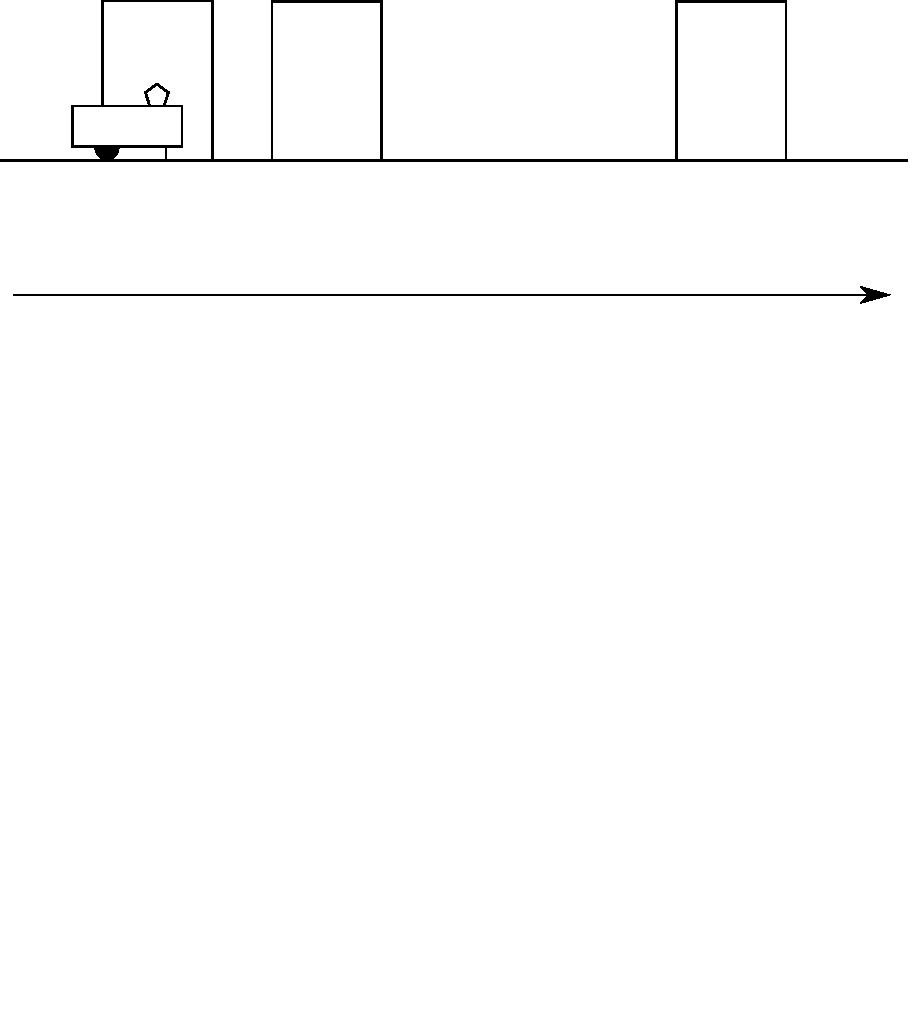
\includegraphics[width=\textwidth]{figs/three_door_example}
    \def\svgwidth{\textwidth}
    \import{./figs/}{three_door_example.pdf_tex}
	\caption{A robot localizing itself using a ``door detector'' in a known map. Top: Upon encountering a door, the robot can be in front of any of the three doors. Middle: When driving to the right, the Gaussian distributions representing its location also shift to the right and widen, representing growing uncertainty. Bottom: After detecting the second door, the robot can discard hypotheses that are not in front of the door and gains certainty on its location. 
	\label{fig:three_door_example}}
\end{figure}

\section{Markov Localization}\label{sec:markovloc}
Calculating the probability to be at a certain location given the likelihood of certain observations is the same as any other conditional probability. There is a formal way to describe such situations: Bayes' Rule (\cref{sec:bayesrule})\index{Bayes' rule}:
\begin{equation}
P(A|B)=\frac{P(A)P(B|A)}{P(B)}
\end{equation}

\subsection{Perception Update}
How does this map into a Localization framework? Let's assume event $A$ is equivalent to being at a specific location $loc$. Let's also assume that event $B$ corresponds to the event of seeing a particular feature $feat$. We can now rewrite Bayes' rule to

\begin{equation}
P(loc|feat)=\frac{P(loc)P(feat|loc)}{P(feat)}
\label{eq:bayesloc}
\end{equation}

Rephrasing Bayes' rule in this way, we can calculate the probability to be at location $loc$, given that we see feature $feat$. This is known as \textsl{Perception Update}\index{Perception Update (Markov Localization)}. For example, $loc$ could correspond to door 1, 2 or 3, and $feat$ could be the event of sensing a door. What do we need to know to make use of this equation?
\begin{enumerate}
\item We need to know the prior probability to be at location loc $P(loc)$
\item We need to know the probability of seeing the feature if we were actually at this location $P(feat|loc)$
\item We need the probability of encountering the feature feat $P(feat)$
\end{enumerate}
Let's start with (3), which might be the most confusing part of information we need to collect. It may make more sense to consider $P(feat)=\sum_{x\in locations}P(feat|x)*P(x)$, the probability that we'd see this feature in a given location for every possible location. It is also common to see this term set to $1$, with $P(loc|feat)$ written as being proportional to the numerator of \cref{eq:bayesloc} instead of equals.
%The answer is simple, it is safe to assume the probability to measure the feature to be simply one ($P(feat)=1$).

The prior probability to be at location  $loc$, $P(loc)$, is called the \index{Belief Model} \textsl{belief model}. In the case of the 3-door example, it is the value of the Gaussian distribution underneath the door corresponding to $loc$.

Finally, we need to know the probability $P(feat|loc)$ of seeing the feature $feat$ given that we are at location $loc$. If your sensor was perfect, this probability is simply 1 if the feature exists at this location, or 0 if the feature cannot be observed at this location. If your sensor is not perfect, $P(feat|loc)$ corresponds to the likelihood of the sensor to see the feature if it exists.

The last missing piece involves deciding how to represent possible locations. In the graphical example in \cref{fig:three_door_example} we assumed Gaussian distributions for each possible location. Alternatively, we can discretize the world into a grid and calculate the likelihood of the robot to be in any of its cells. In our 3-door world, it might make sense to choose grid cells that have the width of a door.

\subsection{Action Update}
One of the assumptions in the above thought experiment was that we know with certainty that the robot moved right. We will now more formally study how to treat uncertainty from motion. Recall that odometry input is just another sensor that we assume to have a Gaussian distribution; if our odometer tells us that the robot traveled a meter, it could have traveled a little less or a little more, with decreasing likelihood the further we get from the given measurement. We can therefore calculate the posterior probability of the robot moving from a position $loc'$ to $loc$ given its odometer input $odo$:

\begin{equation}
P(loc'->loc|odo)=P(loc'->loc)P(odo|loc'->loc)/P(odo)
\end{equation}

This is again Bayes' rule. The unconditional probability $P(loc'->loc)$ is the prior probability for the robot to have been at location $loc'$. The term $ P(odo|loc'->loc)$ corresponds to the probability to get odometer reading $odo$ after traveling from a position $loc'$ to $loc$. If getting a reading of the amount $odo$ is reasonable for the distance from $loc'$ to $loc$ this probability is high. If it is unreasonable, for example if the distance is larger than what is physically possible, this probability should be very low.

As the robot's location is uncertain, the real challenge is now that the robot could have potentially been anywhere to start with. We therefore have to calculate the posterior probability $P(loc|odo)$ for all possible positions $loc'$. This can be accomplished by summing over all possible locations:
\begin{equation}
P(loc|odo)=\sum_{loc'}P(loc'->loc)P(odo|loc'->loc)
\end{equation}
In other words, the law of total probability requires us to consider all possible locations the robot could have ever been at. This step is known as the \textsl{Action Update}\index{Action Update (Markov Localization)}. In practice we don't need to calculate this for all possible locations, but only those that are technically feasible given the maximum speed of the robot. We note also that the sum notation technically corresponds to a convolution (\cref{sec:convolution}) of the probability distribution of the robot's location in the environment with the robot's odometry error probability distribution.

\subsection{Summary and Examples}
We have now learned two methods to update the belief distribution of where the robot could be in the environment. First, a robot can use external landmarks to update its position. This is known as the \textsl{perception update} and relies on exterioception. Second, a robot can observe its internal sensors. This is an example of an \textsl{action update} and relies on proprioception. The combination of action and perception updates is known as \textsl{Markov Localization}\index{Markov Localization}. You can think about the action update as increasing the uncertainty of the robot's position and the perception update as shrinking it. (You can also think about the action update as a discrete version of the error propagation model.) %Also here we are using the robotics kinematic model and the noise model of the odometer to calculate $ P(odo|loc'->loc)$.

\paragraph{Example 1: Topological Map}
This example describes one of the first successful real robot systems that employed Markov Localization in an office environment. The experiment is described in more detail in a 1995 article of AI Magazine\cite{nourbakhsh1995dervish}. The office environment consisted of two rooms and a corridor that can be modeled by a topological map\index{Topological Map} (\cref{fig:dervish_example}). In a topological map, areas that the robot can be in are modeled as vertices, and navigable connections between them are modeled as edges of a graph. The location of the robot can now be represented as a probability distribution over the vertices of  this graph.

\begin{figure}
	\centering
	% 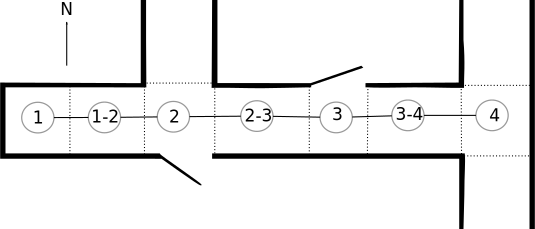
\includegraphics[width=\textwidth]{figs/dervish_example}
    \def\svgwidth{\textwidth}
    \import{./figs/}{dervish_example.pdf_tex}
	\caption{An office environment consisting of two rooms connected by a hallway. A topological map is super-imposed.
	\label{fig:dervish_example}}
\end{figure}

The robot has the following sensing abilities:
\begin{itemize}
    \item It can detect a closed door to its left or right.
    \item It can detect an open door to its left or right.
    \item It can detect whether it is an open hallway.
\end{itemize}

Unfortunately, the robot's sensors are not at all reliable. The researchers have experimentally found the probabilities to obtain a certain sensor response for specific physical positions using their robot in their environment. These values are provided in \cref{tab:dervish_example}.

\begin{table}
\footnotesize
\begin{tabular}{lccccc}
 	& Wall	& Closed dr & Open dr	& Open hwy & Foyer\\
\hline
Nothing detected	& 70\%	& 40\%&	5\%	& 0.1\% & 30\%\\
Closed door detected & 30\% &	60\%& 0\% &0\%	& 5\%\\
Open door detected & 0\%	& 0\%&	90\% & 10\% & 15\%\\
Open hallway detected & 0\% &	 0\%&	0.1\% & 90\% &50\%\\
\hline
\end{tabular}
\normalsize
\caption{Conditional probabilities of the Dervish robot detecting certain features in the Stanford laboratory.\label{tab:dervish_example}}
\end{table}

For example, the success rate to detect a closed door is only 60\%, whereas a foyer looks like an open door in 15\% of the trials. This data corresponds to the conditional probability to detect a certain feature given a certain location.

Consider now the following initial belief state distribution: $p(`1-2')=0.8$ and $p(`2-3')=0.2$. Here, `$1-2$' and `$2-3$' refer to the positions on the topological map in \cref{fig:dervish_example}. For this domain, we are told with certainty that the robot faces east. The robot now drives for a while until it reports ``open hallway on its left and open door on its right''. This actually corresponds to location 2, but the robot can in fact be anywhere. For example there is a 10\% chance that the open door is in fact an open hallway, i.e.\ the robot is really at position 4. How can we calculate the new probability distribution of the robot's location? Here are the possible trajectories that could happen:

The robot could move from $2-3$ to $3$, $3-4$ and finally $4$. We have chosen this sequence as the probability to detect an open door on its right is zero for $3$ and $3-4$, which leaves position $4$ as the only option if the robot has started at $2-3$. In order for this hypothesis to be true, the following events need to have happened, their probabilities are given in parentheses:
\begin{enumerate}
    \item The robot must have started at $2-3$ (20\%)
    \item Not have seen the open door at the left of $3$ (5\%) and not have seen the wall at the right (70\%)
    \item Not have seen the wall to its left (70\%) and not have seen the wall to its right at node $3-4$ (70\%)
    \item Correctly identify the open hallway to its left (90\%) and mistake the open hallway to its right for an open door (10\%)
\end{enumerate}
Together, the likelihood that the robot got from position $2-3$ to position $4$ is therefore given by $0.2\times 0.05 \times 0.7 \times 0.7 \times 0.7 \times 0.9 \times0.1=0.03\%$, that is very unlikely.

The robot could also move from $1-2$ to $2$, $2-3$, $3$, $3-4$ or $4$. We can evaluate these hypotheses in a similar way:
\begin{itemize}
    \item The chance that it correctly detects the open hallway and door at position $2$ is $0.9 \times 0.9$, so the chance to be at position $2$, having started at $1-2$, is $0.8 \times 0.9 \times 0.9=64\%$.
    \item The robot cannot have ended up at position $2-3$, $3$, and $3-4$ because the chance of seeing an open door instead of a wall on the right side is zero in all these cases.
    \item In order to reach position $4$, the robot must have started at $1-2$ has a chance of $0.8$. The robot must not have seen the hallway on its left and the open door to its right when passing position $2$. The probability for this is $0.001 \times 0.05$. The robot must then have detected nothing at $2-3$ ($0.7 \times 0.7$), nothing at $3$ ($0.05 \times 0.7$), nothing at $3-4$ ($0.7 \times 0.7$), and finally mistaken the hallway on its right for an open door at position $4$ ($0.9 \times 0.1$). Multiplied together, this outcome is very unlikely.
\end{itemize}

Given this information, we can now calculate the posterior probability to be at a certain location on the topological map by adding up the probabilities for every possible path to get there.

\paragraph{Example 2: Grid-based Markov Localization}

\begin{figure}
	\centering
	% 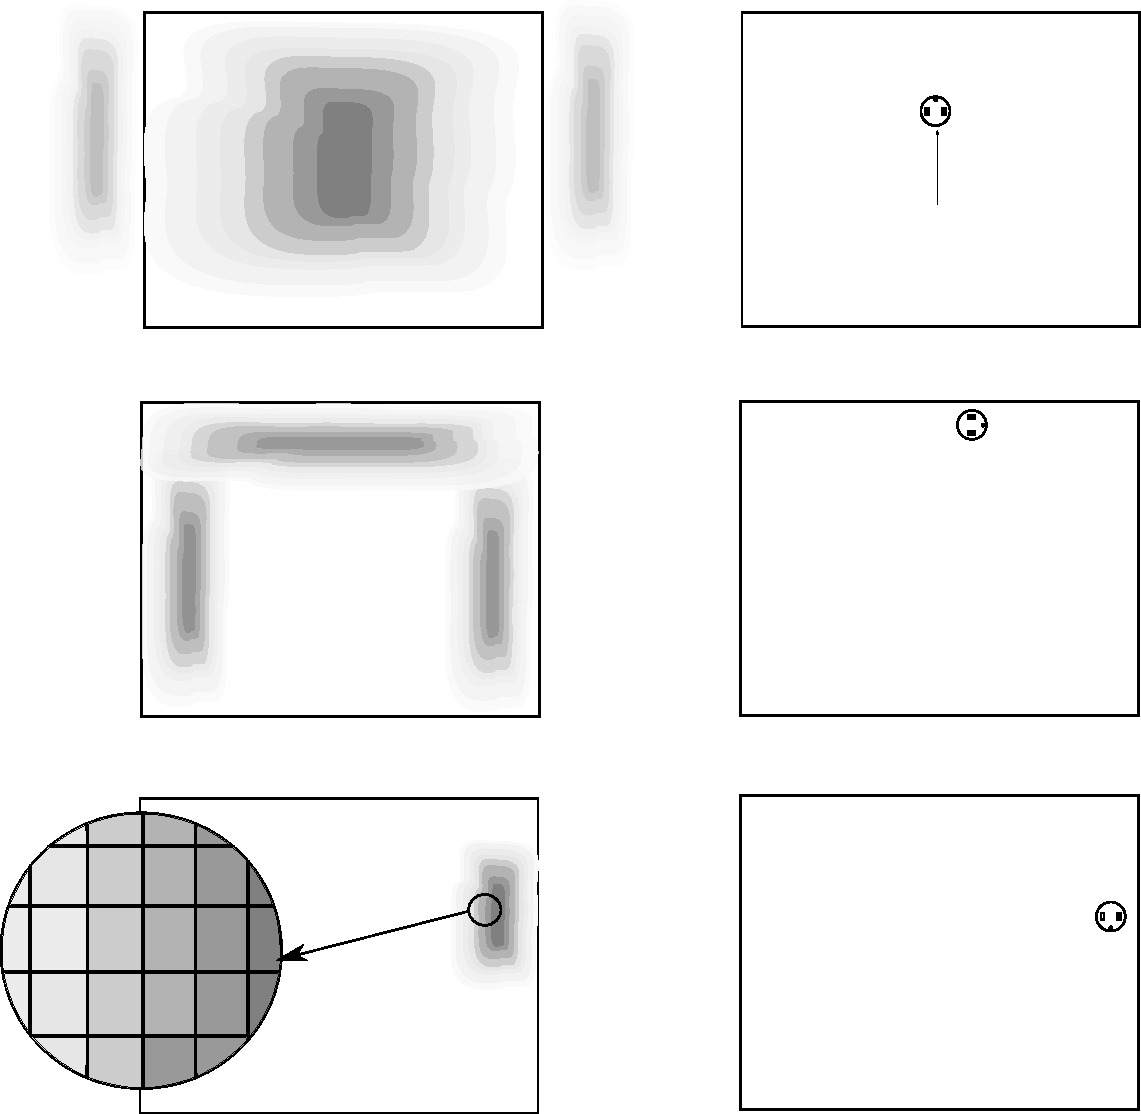
\includegraphics[width=\textwidth]{figs/markov_grid_example}
    \def\svgwidth{\textwidth}
    \import{./figs/}{markov_grid_example.pdf_tex}
	\caption{Markov localization on a grid. The left column shows the likelihood to be in a specific cell as grey value (dark colors correspond to high likelihoods). The right column shows the actual robot location. Arrows indicate previous motion. Initially, the position of the robot is unknown, but recorded upwards motion makes positions at the top of the map more likely. After the robot has encountered a wall, positions away from walls become unlikely. After rightwards and down motions, the possible positions have shrunk to a small area.}
	\label{fig:markov_grid_example}
\end{figure}

Instead of using a coarse topological map, we can also model the environment as a fine-grained grid. Each cell is marked with a probability corresponding to the likelihood of the robot being at this exact location (\cref{fig:markov_grid_example}). We assume that the robot is able to detect walls with some certainty, perhaps with a short-range ultrasonic sensor on the front, back, and sides of the robot. The images in the right column show the actual location of the robot, while the left column shows the probability of the robot being in each grid cell. Initially, the robot does not see a wall and therefore could be almost anywhere. The robot now moves northwards. The action update now propagates the probability of the robot being somewhere north. As soon as the robot encounters the wall, the perception update bumps up the likelihood to be higher in grid cells near walls. As there is some uncertainty associated with the wall detector, the robot will not only have likelihood directly at the wall, but also at other locations --- with decreasing probability --- close by to walls. As the action update involved continuous motion to the north, the likelihood that the robot is close to the south wall is almost zero. The robot then performs a right turn and travels along the wall in the clockwise direction. As soon as it hits the east wall, it is almost certain about its position, which then again decreases as the robot continues to travel.

\section{The Bayes Filter}\index{Bayes Filter}
We have seen how sensor measurements can be formally incorporated into a position estimate using Bayes' rule, which relates the likelihood of being at a certain position given that the robot sees a certain feature to the likelihood of the robot seeing this feature if it were really at the hypothetical location. We have also seen how the robot can use its sensor model to relate its observation with possible positions. 
Its real location is likely to be somewhere between its original belief (based on error propagation) and where the sensor tells it that it is. We will now provide an algorithm for localizing a robot through a multi-hypothesis, iterative process that does not depend on a particular class of motion or sensor model (e.g., the Gaussian noise models used by Kalman Filters).

To formalize our terms and notation, we will describe our robot's motion model as the distribution given by $P(x'|x,u)$, that is, the probability of being in a particular state $x'$ given that we started in state $x$ and executed action $u$. We can describe our sensor model as being characterized by the distribution given by $P(z|x)$, namely the probability that we would see sensor observation $z$ if we were in state $x$. Finally, we will define the probability of being in a particular state $x$ as $P(x)$. 

Our goal with the Bayes filter will be to estimate our robot's state over time ($x_t$, where $t$ indicates timestep) given a history of actions and observations (sensor measurements). To do so, we will compute the posterior probability of our state estimate, also known as \textsl{belief}\index{Belief}, using this history. We define the belief that our robot is in state $x$ at time $t$ given a history of actions ($u_1,...u_t$) and sensor measurements ($z_1,...,z_t$) as:
$$
Bel(x_t) = P(x_t|u_1,z_1,u_2,z_2,...,u_t,z_t)
$$

By leveraging the Markov assumption, that our current state only depends on our previous state $x_{t-1}$ and action $u_t$, we can greatly simplify the computation required. 
$$
P(x_t|x_{0:t-1}, z_{1:t-1}, u_{1:t}) = P(x_t|x_{t-1},u_t)
$$
For example, if we wanted to calculate the probability of an observation $z_t$, we know that the only term that actually matters is the robot's current state (since the other terms don't affect what sensor readings we'd expect to get).
$$
P(z_t|x_{0:t}, z_{1:t-1}, u_{1:t}) = P(z_t|x_t)
$$

We will now derive a recursive definition for belief that makes iteratively computing state belief over a time history of actions and observations tractable. Beginning with our initial definition of belief, we will apply Bayes rule, the Markov property, the law of total probability, and recursion to achieve our goal. We will use $c$ to denote the normalizing constant (from the denominator of Bayes rule), which is the same for all possible $x_t$.
\begin{align}
	Bel(x_t) = {}&  P(x_t|u_1,z_1,...,u_t,z_t)\\
	Bel(x_t) = {}& c * P(z_t|x_t,u_1,z_1,...,u_t,z_t)*P(x_t|u_1,z_1,...,u_t)\\
	Bel(x_t) = {}& c * P(z_t|x_t)*P(x_t|u_1,z_1,...,u_t)\\
	\begin{split}
	Bel(x_t) = {}& c * P(z_t|x_t) *\\&  \sum_{x_{t-1}\in X}P(x_t|u_1,z_1,...,u_t,x_{t-1})*P(x_{t-1}|u_1,z_1,...,z_{t-1},u_t)
	\end{split}\\
	Bel(x_t) = {}& c * P(z_t|x_t)*  \sum_{x_{t-1}\in X}{P(x_t|u_t,x_{t-1})*P(x_{t-1}|u_1,z_1,...,z_{t-1})}\\
	Bel(x_t) = {}& c * P(z_t|x_t) * \sum_{x_{t-1}\in X}{P(x_t|u_t,x_{t-1})*Bel(x_{t-1})}
\end{align}

This final equation is remarkable because it allows us to perform a belief update for a given state by incorporating a sensor measurement and/or a motion prediction based on an action we took. With this formulation, we can define an algorithm for belief updates that takes our current belief, an array of action and observation data, and the set of states that comprise the state space as inputs, returning an updated belief that incorporates this information.

\begin{Verbatim}[commandchars=\\\{\}, codes={\catcode`$=3\catcode`^=7\catcode`_=8}]
BayesFilter(Belief Bel, Data d, Set of States X):
  while d is not empty:
    c = 0
    if (d[0] is a sensor measurement):
      z = d.pop(0)
      for all $x \in X$:
        Bel'(x) = P(z|x)Bel(x)
        c += Bel'(x)
      for all $x \in X$:
        Bel'(x) = $c^{-1}$*Bel'(x)
    elif (d[0] is an action):
      u = d.pop(0)
      for all $x \in X$:
        Bel'(x) = $\sum_{x_{t-1}}P(x|u,x_{t-1})*$Bel$(x_{t-1})$
    Bel = Bel'
  return Bel
\end{Verbatim}

This powerful idea of iteratively incorporating sensor measurements and motion predictions underpins an entire family of state estimation methods. In the sections that follow, we will extend this concept to be applicable in contexts that we often find robots: infinitely large, continuous state spaces that we cannot exhaustively iterate over.

%\section{The Kalman Filter}
%To overcome the limitations of the Bayes filter, we will consider modeling our belief distribution using a family of probability distributions that can be parameterized, as opposed to defining our belief distribution in a discrete point-wise manner. To motivate our choice of distribution family, we turn to the Central Limit Theorem\index{Central Limit Theorem}, which stipulates that random variables that are determined by the sum of lots of small effects are normally distributed. In other words, given an infinite sequence of independent random variables $X_1, X_2, ...$, with $E[X_i]=\mu$ (mean) and $E[X_i-\mu]=\sigma^2$ (variance). Let the value $Z_n$ be defined for $n$ random variables as follows:
%$$
%Z_n = \frac{(X_1+...+X_n)-n\mu}{\sigma\sqrt{n}}
%$$
%As $n\rightarrow \infty$, $Z_n$ is distributed according to the zero-mean, unit-variance Gaussian 
%$\mathcal{N}(0,1)$.\\


\section{Particle Filter}
Although grid-based Markov Localization can provide compelling results, it can be computationally very expensive, in particular when the environment is large and the resolution of the grid is small. This is in part due to the fact that we need to carry the probability to be at a certain location forward for every cell on the grid, regardless of how small this probability is. An elegant solution to this problem is the particle filter. It works as follows:
\begin{enumerate}
\item Represent the robot's position by $N$ particles that are randomly distributed around its estimated initial position. For this, we can either use one or more Gaussian distributions around the initial estimate(s) of where the robot is, or choose an uniform distribution (\cref{fig:particlefilter_example}).
\item Every time the robot moves, we will move each particle in the exact same way, but add noise to each movement much like we would observe on the real robot. Without a perception update, the particles will spread apart farther and farther.
\item Upon a perception event, we evaluate every single particle using our sensor model. What would the likelihood be to have a perception event such as we observed at this location? We can then use Bayes' rule to update each particle's position.
\item Once in a while or during perception events that render certain particles infeasible, particles that have a probability that is too low can be deleted, while those with the highest probability can be replicated.
\end{enumerate}

\begin{figure}[!htb]
	\centering
	% 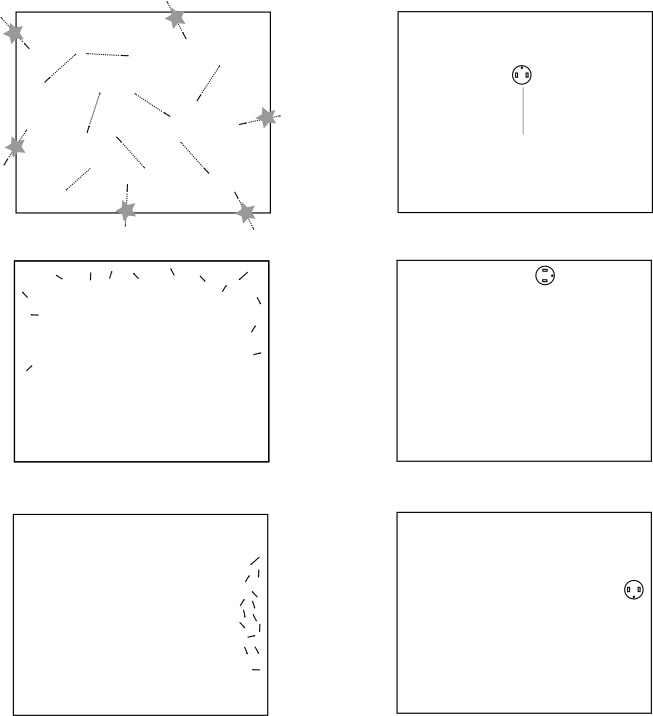
\includegraphics[width=\textwidth]{figs/particlefilter_example}
    \def\svgwidth{0.92\textwidth}
    \import{./figs/}{particlefilter_example.pdf_tex}
	\caption{Particle filter example. Possible positions and orientations of the robot are initially uniformly distributed. Particles move based on the robot's motion model. Particles that would require the robot to move through a wall in absence of a wall perception event are deleted (stars). After a perception event, particles too far from a wall become too unlikely and are resampled to be in the vicinity of a wall. Eventually, the particle filter converges.
	\label{fig:particlefilter_example}}
\end{figure}


\paragraph{Observation}
Let us now assume that we can detect line features $ \boldsymbol{z}_{k,i}=(\alpha_i,r_i)^T$, where $ \alpha$ and $ r$ are the angle and distance of the line from the coordinate system of the robot. These line features are subject to variances $ \sigma_{\alpha,i}$ and $ \sigma_{r,i}$, which make up the diagonal of $ \boldsymbol{R}_{k}$. See the line detection section for a derivation of how angle and distance as well as their variance can be calculated from a laser scanner. The observation is a 2x1 matrix.

\paragraph{Measurement Update}
We assume that we can uniquely identify the lines we are seeing and retrieve their real position from a map that we have been given in advance. This is much easier for unique features, but can also be done for lines by assuming that our error is small enough and we therefore can search through our map and pick the closest lines. As features are stored in global coordinates, we need to transform them into how the robot would see them. In practice this is nothing but a list of lines, each with an angle and a distance, but this time with respect to the origin of the global coordinate system. Transforming them into robot coordinates is straightforward. With  $ \hat{\boldsymbol{x}}_{k}=(x_{k},y_{k},\theta_k)^T$ and $ m_i=(\alpha_i,r_i)$ the corresponding entry from the map, we can write

\begin{equation} h(\hat{\boldsymbol{x}}_{k|k-1})=\left[\begin{array}{c}\alpha_{k,i}\\r_{k,i}\end{array}\right]=h(\boldsymbol{x},m_i)=\left[\begin{array}{c}\alpha_i-\theta\\r_i-(x cos(\alpha_i)+y sin(\alpha_i)\end{array}\right]
\end{equation}

and calculate its Jacobian $ \boldsymbol{H}_{k}$ as the partial derivatives of $ \alpha$ to $ x,y,\theta$ in the first row, and the partial derivatives of $ r$ in the second. How to calculate $ h()$ to predict the radius at which the robot should see the feature with radius $ r_i$ from the map is illustrated in the figure below.


%\begin{mdframed}
%Example on how to predict the distance to a feature the robot would see given its estimated position and its known location from a map.
%\end{mdframed}

\paragraph{Matching}
We are now equipped with a measurement $ \boldsymbol{z}_k$ and a prediction $ h(\hat{\boldsymbol{x}}_{k|k-1})$ based on all features stored in our map. We can now calculate the innovation
\begin{equation}
\tilde{\boldsymbol{y}}_{k}=\boldsymbol{z}_{k}-h(\hat{\boldsymbol{x}}_{k|k-1})
\end{equation}

which is simply the difference between each feature that we can see and those that we predict from the map. The innovation is again a 2x1 matrix.

A major strength of particle filters is that they are non-parametric estimators of arbitrary probability distributions, and thus are able to accommodate non-linear functions that Kalman Filters cannot. However, this is not the only algorithm available for utilizing non-linear motion and sensor models for state estimation. We now introduce a modification to the Kalman Filter enabling the use of non-linear models.


\section{Extended Kalman Filter}\label{sec:EKF}
In contrast to the linear models required of the Kalman Filter, in the Extended Kalman Filter the state transition and observation models do not need to be linear functions of the state but may instead be any function so long as it's differentiable. The action prediction step looks as follows:
\begin{equation}
\hat{\boldsymbol{x}}_{k'|k-1} = f(\hat{\boldsymbol{x}}_{k-1}, \boldsymbol{u}_{k-1})
\end{equation}
Here $ f()$ is a function of the previous state $ \boldsymbol{x}_{k-1}$ and control input $ \boldsymbol{u}_{k-1}$. A good example for such an equation is the odometry update we are already familiar with. Here, $ f()$ is a function describing the forward kinematics of the robot, $ \boldsymbol{x}_k$ its position and $ \boldsymbol{u}_k$ the wheel-speed we set.

Sticking with our well known example, we can also calculate the covariance matrix of the robot position

\begin{equation}
\boldsymbol{P}_{k'|k-1} = \nabla_{x,y,\theta}f \boldsymbol{P}_{k-1|k-1}\nabla_{x,y,\theta}f^T + \nabla_{\Delta_{r,l}}f\boldsymbol{Q}_{k-1}\nabla_{\Delta_{r,l}}f^T
\end{equation}

where $ \boldsymbol{Q}_k$ was the covariance matrix of the wheel-slip and the Jacobian matrices of the forward kinematic equations $ f()$ with respect to the robot's position (indicated by the index $ x,y,\theta$) and with respect to the wheel-slip of the left and right wheel.

The perception update step now looks as follows:

\begin{eqnarray}
\hat{\boldsymbol{x}}_{k|k'} &=& \hat{\boldsymbol{x}}_{k'|k-1} + \boldsymbol{K}_{k'}\tilde{\boldsymbol{y}}_{k'}\\
\boldsymbol{P}_{k|k'} &=& (I - \boldsymbol{K}_{k'} {\boldsymbol{H}_{k'}}) \boldsymbol{P}_{k'|k-1}
\end{eqnarray}

We are calculating everything twice: once we update from $ k-1$ to an intermediate result $ k'$ during the action update using our motion model, we obtain the final result after performing the perception update where we go from $ k'$ to $ k$.

We need to calculate three additional variables:
\begin{enumerate}
\item The innovation $ \tilde{\boldsymbol{y}}_{k}=\boldsymbol{z}_{k}-h(\hat{\boldsymbol{x}}_{k|k-1})$
\item The covariance of the innovation $\boldsymbol{S}_{k}={\boldsymbol{H}_{k}}\boldsymbol{P}_{k|k-1}{\boldsymbol{H}_{k}^\top}+\boldsymbol{R}_{k}$
\item The (near-optimal)  Kalman gain $ \boldsymbol{K}_{k}=\boldsymbol{P}_{k|k-1}{\boldsymbol{H}_{k}^\top}\boldsymbol{S}_{k}^{-1}$
\end{enumerate}
Here $ h()$ is the observation model and $ \boldsymbol{H}$ its Jacobian. How these equations are derived is involved (and is one of the fundamental results in control theory), but the idea is the same as introduced above: we wish to minimize the error of the prediction.

\subsection{Odometry using the Kalman Filter}
We will show how a mobile robot equipped with a laser scanner that has a map of the environment can correct its position estimate by relying on unreliable odometry and unreliable sensing, in an optimal way.
Whereas the update step is equivalent to forward kinematics and error propagation that we have seen before, the observation model and calculating the ``innovation'' require additional steps to perform odometry.

\paragraph{1. Prediction}
We assume for now that the reader is familiar with calculating $ \hat{\boldsymbol{x}}_{k'|k-1}=f(x,y,\theta)^T$ and its variance $ \boldsymbol{P}_{k'|k-1}$. Here, $ \boldsymbol{Q}_{k-1}$, the covariance matrix of the wheel-slip error,  is given by
\begin{equation}
\boldsymbol{Q}_{k-1}=\left[\begin{array}{cc}k_r|\Delta s_r & 0\\0 & k_l|\Delta s_l|\end{array}\right]
\end{equation}
where $\Delta s_l$ and $\Delta s_r$ is the wheel movement of the left and right wheel and $k_l$ and $k_r$ are constants. Refer to the odometry lab for detailed derivations of these calculations and how to estimate $ k_r$ and $ k_l$.  The state vector $ \boldsymbol{\hat{x}_{k'|k-1}}$ is a 3$\times$1 vector, the covariance matrix $ \boldsymbol{P_{k'|k-1}}$ is a 3$\times$3 matrix, and $ \nabla_{\Delta_{r,l}}$ that is used during error propagation is a 3$\times$2 matrix. See the error propagation section for details on how to calculate $ \nabla_{\Delta_{r,l}}$.

%% crh: I don't know who's todo this was, but it wasn't mine... commenting for now.

%\td{EDIT THIS FROM MAPPING TO LOCALIZATION ONLY}
%i%\paragraph{2. Observation}
%Let us now assume that we can detect the motion of the robot through an optical flow sensor.
\paragraph{2. Observation}
Let us now assume that we can detect line features $ \boldsymbol{z}_{k,i}=(\alpha_i,r_i)^T$, where $ \alpha$ and $ r$ are the angle and distance of the line from the coordinate system of the robot. These line features are subject to variances $ \sigma_{\alpha,i}$ and $ \sigma_{r,i}$, which make up the diagonal of $ \boldsymbol{R}_{k}$. See the line detection section for a derivation of how angle and distance as well as their variance can be calculated from a laser scanner. The observation is a 2$\times$1 matrix (representing angle and distance).

\paragraph{3. Measurement Update}
We assume that we can uniquely identify the lines we are seeing and retrieve their real position from a map. This is much easier for unique features, but can also be done for lines by assuming that our error is small enough and that we can search through our map and pick the closest lines. As features are stored in global coordinates, we need to transform them into how the robot would see them. In practice this is nothing but a list of lines specified with respect to the origin of the global coordinate system, each with an angle and a distance. Transforming them into robot coordinates is straightforward. With  $ \hat{\boldsymbol{x}}_{k}=(x_{k},y_{k},\theta_k)^T$ and $ m_i=(\alpha_i,r_i)$ the corresponding entry from the map, we can write

\begin{equation} h(\hat{\boldsymbol{x}}_{k|k-1})=\left[\begin{array}{c}\alpha_{k,i}\\r_{k,i}\end{array}\right]=h(\boldsymbol{x},m_i)=\left[\begin{array}{c}\alpha_i-\theta\\r_i-(x cos(\alpha_i)+y sin(\alpha_i)\end{array}\right]
\end{equation}

and calculate its Jacobian $ \boldsymbol{H}_{k}$ as the partial derivatives of $ \alpha$ to $ x,y,\theta$ in the first row, and the partial derivatives of $ r$ in the second. How to calculate $ h()$ to predict the radius at which the robot should see the feature with radius $ r_i$ from the map is illustrated in the figure below.


%\begin{mdframed}
%Example on how to predict the distance to a feature the robot would see given its estimated position and its known location from a map.
%\end{mdframed}

\paragraph{4. Matching}
We are now equipped with a measurement $ \boldsymbol{z}_k$ and a prediction $ h(\hat{\boldsymbol{x}}_{k|k-1})$ based on all features stored in our map. We can now calculate the innovation
\begin{equation}
\tilde{\boldsymbol{y}}_{k}=\boldsymbol{z}_{k}-h(\hat{\boldsymbol{x}}_{k|k-1})
\end{equation}

which is simply the difference between each feature that we can actually see (our sensor measurement) and the measurement values that we would expect if making a prediction using the map (not using our sensors). The innovation is again a 2x1 matrix.

\paragraph{5. Estimation}
We now have all the ingredients to perform the perception update step of the Kalman filter:

\begin{eqnarray}
\hat{\boldsymbol{x}}_{k|k'} &=& \hat{\boldsymbol{x}}_{k'|k-1} + \boldsymbol{K}_{k'}\tilde{\boldsymbol{y}}_{k'}\\
\boldsymbol{P}_{k|k'} &=& (I - \boldsymbol{K}_{k'} {\boldsymbol{H}_{k'}}) \boldsymbol{P}_{k'|k-1}
\end{eqnarray}

It will provide us with an update of our position that fuses our odometry input and the information that we can extract from features in the environment in a way that takes into account their variances. That is, if the variance of your previous position is high (because you have no idea where you are), but the variance of your measurement is low (maybe from a GPS or a highly recognizable symbol on the wall), the Kalman filter will put more emphasis on your sensor. If your sensors are poor (maybe because you cannot tell different lines/walls apart), more emphasis will be placed on the odometry.

As the state vector is a 3$\times$1 vector and the innovation a 2$\times$1 matrix, the Kalman gain must be a 3$\times$2 matrix. This can also be seen when looking at the covariance matrix that must come out as a 3x3 matrix, and knowing that the Jacobian of the observation function is a 2$\times$3 matrix. We can now calculate the covariance of the innovation and the Kalman gain using

\begin{eqnarray}
\boldsymbol{S}_{k}&=&{\boldsymbol{H}_{k}}\boldsymbol{P}_{k|k-1}{\boldsymbol{H}_{k}^\top}+\boldsymbol{R}_{k}\\
\boldsymbol{K}_{k}&=&\boldsymbol{P}_{k|k-1}{\boldsymbol{H}_{k}^\top}\boldsymbol{S}_{k}^{-1}
\end{eqnarray}



\section{Summary: Probabilistic Map based localization}\label{sec:pmbl}
In order to localize a robot using a map, we need to perform the following steps:
\begin{enumerate}
\item Calculate an estimate of our new position using the forward kinematics and knowledge of the wheel-speeds that we sent to the robot until the robot encounters some uniquely identifiable feature.
\item Calculate the relative position of the feature (a wall, a landmark or beacon) to the robot.
\item Use knowledge of where the feature is located in global coordinates to predict what the robot should see.
\item Calculate the difference between what the robot actually sees and what it believes it should see (e.g.\ using a Kalman filter).
\item Use the result from (4) to update its belief by weighing each observation against its variance.
\end{enumerate}

Steps 1-2 are based on the sections on ``Forward Kinematics'' and ``Line detection''. Step 3 uses again simple forward kinematics to calculate the position of a feature stored in global coordinates in a map in robot coordinates. Step 4 is a simple subtraction of what the sensor sees and what the map says. Step 5 may induce the Kalman filter, or an error minimization constraint. %, which we will describe here. Its derivation is involved, but its intuition is simple: why just averaging between where I think I am and what my sensors tell me, if my sensors are much more reliable and should carry much higher weight?


\section*{Take home lessons}
\begin{itemize}
\item If the robot has no additional sensors and its odometry is noisy, error propagation will lead to ever increasing uncertainty of a robot's position regardless of using Markov localization or the Kalman filter.
\item Once the robot is able to sense features with known locations, Bayes' rule can be used to update the posterior probability of a possible position. The key insight is that the conditional probability to be at a certain position given a certain observation can be inferred from the likelihood to actually make this observation given a certain position.
\item A complete solution that performs this process for discrete locations is known as Markov Localization.
\item The Extended Kalman Filter is the optimal way to fuse observations of different random variables that are Gaussian distributed.
%It is derived by minimizing the least-square error between prediction and real value.
\item Possible random variables could be the estimate of your robot position from odometry and observations of static beacons with known location (but uncertain sensing) in the environment.
\item In order to take advantage of the approach, you will need differentiable functions that relate measurements to state variables as well as an estimate of the covariance matrix of your sensors.
\item An approximation that combines benefits of Markov Localization (multiple hypothesis) and the Kalman filter (continuous representation of position estimates) is the Particle filter.
\end{itemize}

\section*{Exercises}\small
\begin{enumerate}
\item Assume that the ceiling is equipped with infrared markers that the robot can identify with some certainty. Your task is to develop a probabilistic localization scheme, and you would like to calculate the probability $p(marker|reading)$ to be close to a certain marker given a certain sensing reading and information about how the robot has moved.
\begin{enumerate}
\item Derive an expression for $p(marker|reading)$ assuming that you have an estimate of the probability to correctly identify a marker $p(reading|marker)$ and the probability $p(marker)$ of being underneath a specific marker.
\item Now assume that the likelihood that you are reading a marker correctly is 90\%, that you get a wrong reading is 10\%, and that you do not see a marker when passing right underneath it is 50\%. Consider a narrow corridor that is equipped with 4 markers. You know with certainty that you started from the entry closest to marker 1 and move right in a straight line. The first reading you get is ``Marker 3''. Calculate the probability to be indeed underneath marker 3.
\item Could the robot also possibly be underneath marker 4?
\end{enumerate}
\end{enumerate}\normalsize
